\documentclass[10pt,a4paper]{article}
\usepackage{a4wide}
\usepackage{enumerate}
\usepackage{enumitem}
\usepackage{pcptex}
\usepackage{xspace}
\usepackage[toc,page]{appendix}
\usepackage{algorithm}
\usepackage[noend]{algpseudocode}
\usepackage{hyperref}
\usepackage{xcolor}
\usepackage{tikz}
\usepackage{pgfplots}

\renewcommand{\arraystretch}{1.2}

\definecolor{links}{HTML}{2A1B81}
\hypersetup{colorlinks,linkcolor=,urlcolor=links}

\makeatletter
\def\BState{\State\hskip-\ALG@thistlm}
\makeatother

\setlength{\parindent}{0pt}


\begin{document}

\pptitle{A High Performance Implementation of the 2D N-Body Gravitational problem: Benchmark of the Barnes-Hut algorithm compared to the Brute-Force algorithm.}

\ppintro{Gael Lederrey}{EPFL-CSE}{gael.lederrey@epfl.ch}{Only PI}{June 10, 2016}{June 24, 2016}{Deneb}{NBODY-BHVSBF}

\ppabstract{The n-Body problem has been well studied by many scientists in many different fields such as atoms simulation or astrophysics. In this project, we present the implementation of the Barnes-Hut algorithm. A distributed memory version using the MPI library will also be presented. A benchmark comparison is done with the Brute-Force algorithm, serial and parallel versions. The whole project can be found at this url: \href{https://github.com/glederrey/nBody-PHPC-2016-EPFL}{https://github.com/glederrey/nBody-PHPC-2016-EPFL}}

\section{Scientific Background}

\subsection{Gravitation} 

The n-Body problem covers the whole scale of science from the subatomic particles to the gigantic galaxies. In this project, we decided to take the Gravitional n-Body problem as a real case study. The force\cite{grav} of a body 1 on a body 2 is given by:
\begin{equation}
\vec{F}_{1\rightarrow 2} = G\cdot\frac{m_1m_2(\vec{x}_2-\vec{x}_1)}{\Vert \vec{x}_2-\vec{x}_1\Vert^3}
\end{equation}
where $G$ is the gravitational constant and is equal to $6.674 \cdot 10^{-11}~[Nm^2kg^{-2}]$, $m_i$ are their masses and $\vec{x}_i$ their positions. As we can see with this equation, the force decreases proportionally to $1/r^2$, $r$ being the distance between the two bodies. Therefore, the force between two far bodies is small.

\subsection{Algorithms}

In order to solve the n-Body Gravitational problem, there exists a really simple algorithm called Brute-Force. It consists in looping over all bodies and inside this loop, a second traverses all bodies again.

\begin{algorithm}
\caption{Brute-Force}\label{bf}
\begin{algorithmic}[1]
\State $n$ = Number of bodies
\State Initialize $n$ bodies
\While {$t < t_{end}$}
\For {$i = 1 \textit{ to } n$} 
\For {$j = 1 \textit{ to } n$}
\State Apply forces from body $j$ on body $i$
\EndFor
\EndFor
\For {$k = 1 \textit{ to } n$}
\State Update the body $k$
\EndFor
\EndWhile
\end{algorithmic}
\end{algorithm}

We can clearly see that the complexity to compute all forces is $\mathcal{O}(n^2)$. Updating the bodies will take only $\mathcal{O}(n)$ time. It just consists of looping on all the bodies and adding $v\cdot dt$ to the position and $a\cdot dt$ to the speed. But most of the time will be spent in the calculation of the forces. For a very large number of bodies this algorithm will be very slow. Therefore another algorithm can be used: Barnes-Hut\cite{bh}.

The main idea of the Barnes-Hut algorithm is to approximate interactions between bodies which are far away from each other by grouping bodies together. They way to group bodies together is to use their center of mass. On way to implement this is to use a quadtree. Each leaves of the quadtree contains at max one body. Therefore, the height of the tree is approximately $\log(n)$,  $n$ is the number of bodies. All the parents leaves contain the information about the center of mass of the children nodes. With this trick, the algorithm will only compute the forces between a body and the center of mass of the far bodies. The aggregation is done using a precision parameter $\theta$.  The pseudo-code is given below:
\begin{algorithm}
\caption{Barnes-Hut}\label{bh}
\begin{algorithmic}[1]
\State $n$ = Number of bodies
\State Initialize $n$ bodies
\While {$t < t_{end}$}
\For {$i = 1 \textit{ to } n$} 
\State	Add body $i$ in the tree
\EndFor
\For {$j = 1 \textit{ to } n$} 
\State	Compute all the forces applied to body $j$.
\EndFor	
\For {$k = 1 \textit{ to } n$}
\State Update the body $k$
\EndFor
\EndWhile
\end{algorithmic}
\end{algorithm}

Adding a body in the tree takes $\mathcal{O}(\log n)$ time (height of the tree). Therefore, adding all the bodies will take $\mathcal{O}(n\log n)$ time. The calculation of the forces will take $\mathcal{O}(n) \times \mathcal{O}(\log n) = \mathcal{O}(n\log n)$ time. And finally, updating the bodies will take $\mathcal{O}(n)$ time. Therefore, this algorithm will take $\mathcal{O}(n\log n)$ time which is much faster than the Brute-Force algorithm for a high number of bodies.
\\\\
If we use a parallel version of these algorithms, we will have to send the bodies to the other process. Since each body needs to compute its forces with all the other bodies, the process will exchange all $n$ bodies. This means that the communication takes $\mathcal{O}(n)$ time.

\subsection{Too close and too far?} 
Two problems occur with the n-Body problem:
\begin{itemize}
\item What do we do when a body is moving too far form the other bodies?
\item What do we do when two bodies are really close? 
\end{itemize} 

We decided to address these two problems in a very simple manner. First, we define a maximum and minimum distance. We use the maximum distance such that the root node of the tree has a height and a width of two times this maximum distance. If a body is outside of this root node, then we delete it. And if two bodies have a distance smaller than the minimum distance, we combine them using a perfect inelastic collision, {\it i.e.} the mass of the new body will me the sum of the two colliding bodies and the speed will be:
\[
\vec{v} = \frac{m_1\cdot\vec{v}_1 + m_2\cdot\vec{v}_2}{m_1+m_2}
\]

\section{Project Description}

In this project we want to implement a high performance version of the Barnes-Hut algorithm in C++~\cite{c++}. A simple version of the Brute-Force algorithm will also be implemented to be used as a benchmark for the Barnes-Hut algorithm. At the end, four different codes will be produced:
\begin{itemize}
\item Serial version of the Brute-Force algorithm
\item Distributed memory version, using MPI~\cite{mpi}, of the Brute-Force algorithm
\item Serial version of the Barnes-Hut algorithm
\item Distributed memory version, using MPI, of the Barnes-Hut algorithm
\end{itemize}
The three first codes will be used as benchmark for the distributed memory version of the Barnes-Hut algorithm. Indeed, to prove that this version is the fastest, we need to make sure it surpasses the Brute-Force algorithm. 
\\\\
For the two distributed memory codes, we apply Amdahl's law. We will then compare the strong scaling and the weak scaling.

\section{Implementations}

These four applications are implemented in C++. As it was said in the previous section, the distributed memory versions use the MPI library. Everything has been compiled using \verb+gcc+ version 4.8.4. The codes have been debugged using the general debugger \verb+gdb+, and \verb+valgrind+ has been used to remove all the memory leaks. 

\subsection{Optimization}

For each of the codes, we compile it once without using any optimization flags and once with the following two flags: \verb+-Ofast+ and \verb+-ftree-vectorize+.

\subsubsection{Brute-Force}

Not much efforts were put onto the optimization of the Brute-Force algorithm since it exists only for a benchmark purpose. For the MPI version of the code, the first (outer) loop is divided into the number of processes. The second (inner) loop is still on the $n$ bodies. After updating the bodies, we use the function \verb+Allgatherv+ of MPI to distribute the new bodies to all the process.

\subsubsection{Barnes-Hut}

For the Barnes-Hut algorithm, we first assign each node to a process in order to keep a good load-balancing. This part is serial. Then, we can calculate the forces and update the bodies in the nodes belonging to its process. Then, we used the function \verb+Allgatherv+ of MPI to distribute the new bodies to all the process. Finally, we can reconstruct the tree. We did not implement a heuristic for the construction of the tree. But it can be a good idea for future improvement since this step can take some time.

\section{Computational time}

In this section, we want to show that the Brute-Force algorithm is in $\mathcal{O}(n^2)$ and that the Barnes-Hut algorithm is in $\mathcal{O}(n\log n)$. In Figure \ref{fig:algo_time}, the average iteration time taken by the two algorithms are shown for different number of bodies. Different values for the precision parameter $\theta$ were used. We can clearly see that the Brute-Force algorithm has the same slope as the red line. We can also see that the Barnes-Hut algorithm with $\theta=0$ has the same slope. This is normal since it doesn't aggregate any bodies. But if $\theta>0$, we can see that the slope becomes the same as the red dotted line for $\mathcal{O}(n\log n)$, especially with a large number of bodies. Therefore, the experimental computation times correspond to the theoretical ones.

\begin{figure}[H]
\centering
% This file was created by matlab2tikz.
% Minimal pgfplots version: 1.3
%
%The latest updates can be retrieved from
%  http://www.mathworks.com/matlabcentral/fileexchange/22022-matlab2tikz
%where you can also make suggestions and rate matlab2tikz.
%
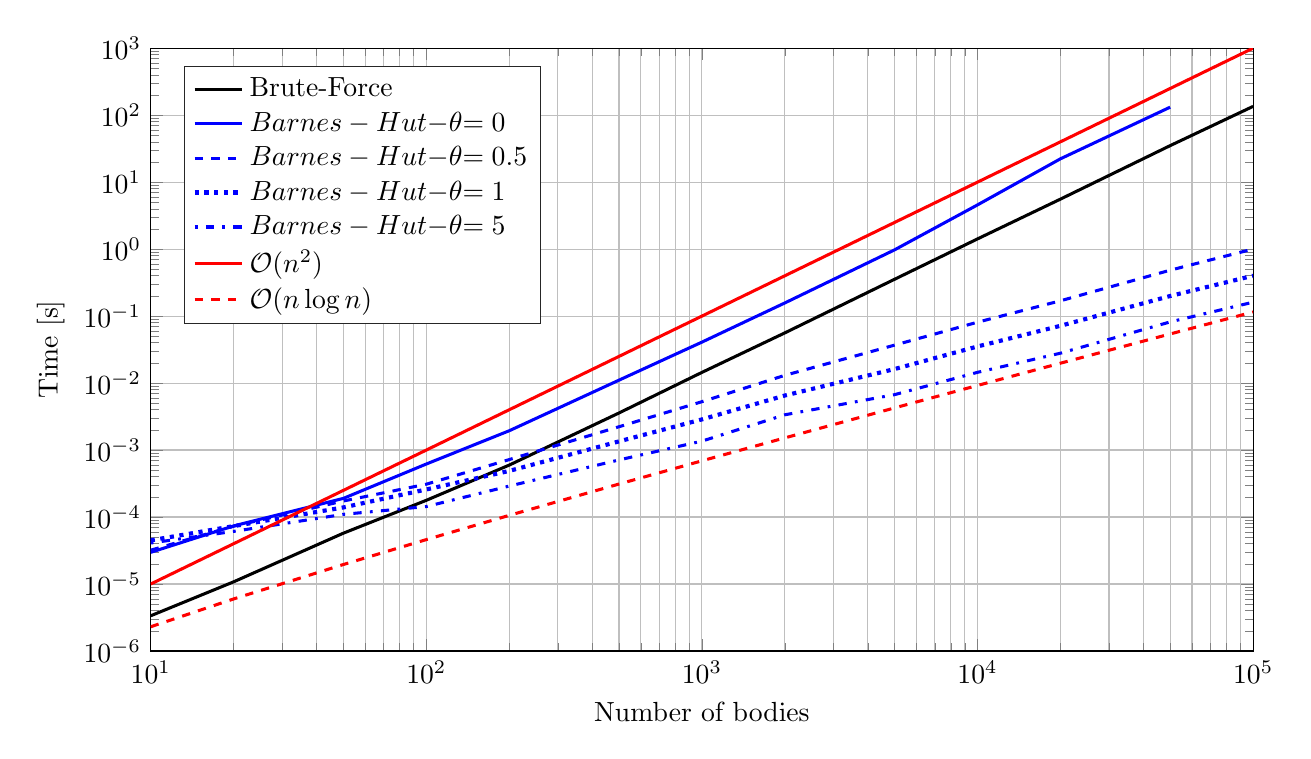
\begin{tikzpicture}

\begin{axis}[%
width=14cm,
height=3.014201in,
at={(0.819271in,0.473819in)},
scale only axis,
xmode=log,
xmin=10,
xmax=100000,
xminorticks=true,
xlabel={Number of bodies},
xmajorgrids,
xminorgrids,
ymode=log,
ymin=1e-06,
ymax=1000,
%yminorticks=true,
ylabel={Time [s]},
ymajorgrids,
%yminorgrids,
legend style={at={(0.03,0.97)},anchor=north west,legend cell align=left,align=left,draw=white!15!black}
]
\addplot [color=black,solid,line width=1.1pt]
  table[row sep=crcr]{%
10	3.35799999999999e-06\\
20	1.0792e-05\\
50	5.73950000000003e-05\\
100	0.000177757000000002\\
200	0.000596881999999996\\
500	0.003575887\\
1000	0.01443757\\
2000	0.05619261\\
5000	0.35453151\\
10000	1.42079354\\
20000	5.57831678947368\\
50000	35.0699816\\
100000	135.2261985\\
};
\addlegendentry{Brute-Force};

\addplot [color=blue,solid,line width=1.1pt]
  table[row sep=crcr]{%
10	2.9745490981964e-05\\
20	7.37354709418837e-05\\
50	0.000189899799599199\\
100	0.000618909819639278\\
200	0.00194345390781563\\
500	0.0110494198396794\\
1000	0.0408762741116751\\
2000	0.157240964467005\\
5000	0.9746818125\\
10000	4.573282625\\
20000	22.304639\\
50000	131.6148535\\
};
\addlegendentry{$\text{Barnes-Hut - }\theta\text{ = 0}$};

\addplot [color=blue,dashed,line width=1.1pt]
  table[row sep=crcr]{%
10	3.19959919839679e-05\\
20	7.29919839679361e-05\\
50	0.000173497995991983\\
100	0.000309158316633266\\
200	0.000721342685370745\\
500	0.00222753907815631\\
1000	0.00527390355329949\\
2000	0.013051614213198\\
5000	0.0368562081218274\\
10000	0.0810765816326531\\
20000	0.169263326530612\\
50000	0.4844115\\
100000	1.002134125\\
};
\addlegendentry{$\text{Barnes-Hut - }\theta\text{ = 0.5}$};

\addplot [color=blue,dotted,line width=1.5pt]
  table[row sep=crcr]{%
10	4.48386773547096e-05\\
20	7.32244488977956e-05\\
50	0.000139150300601203\\
100	0.000258080160320643\\
200	0.000488356713426856\\
500	0.00134697194388778\\
1000	0.00286829441624366\\
2000	0.00652302538071066\\
5000	0.0161893299492386\\
10000	0.0351909795918367\\
20000	0.0716242653061224\\
50000	0.19952875\\
100000	0.400152875\\
};
\addlegendentry{$\text{Barnes-Hut - }\theta\text{ = 1}$};

\addplot [color=blue,dash pattern=on 1pt off 3pt on 3pt off 3pt,line width=1.1pt]
  table[row sep=crcr]{%
10	4.0967935871744e-05\\
20	6.10551102204412e-05\\
50	0.000109647294589179\\
100	0.000143380761523046\\
200	0.000290100200400802\\
500	0.000711711422845691\\
1000	0.00135943147208122\\
2000	0.00336177157360406\\
5000	0.00671562436548223\\
10000	0.0144679387755102\\
20000	0.0279377551020408\\
50000	0.081869875\\
100000	0.161289625\\
};
\addlegendentry{$\text{Barnes-Hut - }\theta\text{ = 5}$};

\addplot [color=red,solid,line width=1.1pt]
  table[row sep=crcr]{%
10	1e-05\\
20	4e-05\\
50	0.00025\\
100	0.001\\
200	0.004\\
500	0.025\\
1000	0.1\\
2000	0.4\\
5000	2.5\\
10000	10\\
20000	40\\
50000	250\\
100000	1000\\
};
\addlegendentry{$\mathcal{O}(n^2)$};

\addplot [color=red,dashed,line width=1.1pt]
  table[row sep=crcr]{%
10	2.30258509299405e-06\\
20	5.99146454710798e-06\\
50	1.95601150271407e-05\\
100	4.60517018598809e-05\\
200	0.000105966347330961\\
500	0.00031073040492111\\
1000	0.000690775527898214\\
2000	0.00152018049190842\\
5000	0.00425859659570812\\
10000	0.00921034037197618\\
20000	0.0198069751050723\\
50000	0.0540988914220514\\
100000	0.115129254649702\\
};
\addlegendentry{$\mathcal{O}(n \log n)$};

\end{axis}
\end{tikzpicture}%
\caption{\label{fig:algo_time} Average time of the main iteration for the Brute-Force and the Barnes-Hut algorithms. Different values for the precision, $\theta$, have been used. The theoretical times are given in red.}
\end{figure}

An interesting fact is to see that for a small number of bodies, the Brute-Force algorithm is faster than the Barnes-Hut algorithm. This may be due to the optimization made by the compiler and the implementation of the Barnes-Hut algorithm. However, with $10^5$ bodies, we see that the Barnes-Hut algorithm, $\theta=1$, is more than $1000$ times faster than the Brute-Force algorithm. For the rest of the project, we will always use $\theta=1$.

\section{Amdahl's law}

Amdahl's law is given by:
\begin{equation}
S_{p} = \frac{1}{\alpha + \frac{1-\alpha}{p}}
\end{equation}
where $S_{p}$ is the theoretical speedup, $1-\alpha$ is the parallelizable part of the code and $p$ is the number of processors. Ideally, we should have $S_p = p$ but this does not happen in reality. To compute Amdahl's law, we don't take into account the time taken to load the initial data. It can take some time but it is done only once. On a long simulation, this time will be negligible.

\subsection{Brute-Force}

In the Brute-Force algorithm, everything can be parallelized except the communication between the process. Therefore we can expect a speedup very close to the perfect speedup, {\it i.e.} $S_p = p$.

\subsection{Barnes-Hut}

In the Barnes-Hut algorithm, the communication between the process is serial. The assignment of the nodes to the processes needs to be done in serial, so does the construction of the tree. All processes will do these two things. The construction of the tree can take a bit of time, therefore, we will except a smaller speedup.

\subsection{Results}

Table \ref{tab:amdahl} presents different times taken by the code for the Brute-Force and the Barnes-Hut algorithms. The different times are: $\overline{t}_{it}$ for the average time of the iteration, $\overline{t}_{c}$ for the average time taken for the communication, $\overline{t}_{a}$ for the average time taken for the assignment of the nodes to the process and $\overline{t}_{b}$ for the average time taken for building the tree. The time $\overline{t}_{it}$ takes into account all other times and in addition the parallel times: computing the forces and updating the bodies. Therefore we can easily determine $\alpha$, the percentage of serial part of the code, easily. It is given by:
\[
\alpha_{\text{bf}} = \frac{\overline{t}_{c}}{\overline{t}_{it}} \qquad\qquad \text{or} \qquad\qquad \alpha_{\text{bh}} = \frac{\overline{t}_{c} + \overline{t}_{a} + \overline{t}_{b}}{\overline{t}_{it}}
\]

\begin{table}[h]
\centering
\begin{tabular}{|c||c|c|c|c|c||c|}
\hline
Algorithm & $n$ & $\overline{t}_{it}~[s]$ & $\overline{t}_{c}~[s]$ & $\overline{t}_{a}~[s]$ & $\overline{t}_{b}~[s]$ & $\alpha$ \\
\hline \hline
\multirow{3}{*}{Brute-Force} & $10^4$ & $1.08$ & $2.87\cdot 10^{-5}$ & / & / & $2.66\cdot10^{-5}$ \\ \cline{2-7}
& $10^5$ & $1.08\cdot10^2$ & $1.52\cdot 10^{-4}$ & / & / & $1.41\cdot10^{-6}$ \\ \cline{2-7}
& $10^6$ & $1.08\cdot10^4$ & $4.07\cdot 10^{-3}$ & / & / & $3.77\cdot10^{-7}$ \\ \hline \hline
\multirow{3}{*}{Barnes-Hut} & $10^4$ & $3.04\cdot10^{-2}$ & $4.95\cdot 10^{-5}$ & $8.39\cdot10^{-7}$ & $5.45\cdot10^{-3}$ & $1.81\cdot10^{-1}$ \\ \cline{2-7}
& $10^5$ & $3.70\cdot10^{-1}$ & $6.49\cdot10^{-4}$ & $2.64\cdot10^{-6}$ & $7.24\cdot10^{-2}$ & $1.97\cdot10^{-1}$ \\ \cline{2-7}
& $10^6$ & $4.39$ & $9.612\cdot10^{-3}$ & $2.57\cdot10^{-6}$ & $7.93\cdot10^{-1}$ & $1.82\cdot10^{-1}$ \\ \hline
\end{tabular}
   \caption{Times used to compute the serial part of the code for Amdahl's law.}
   \label{tab:amdahl}  
\end{table}

Finally, given the serial fraction of the code $\alpha$, we can plot Amdahl's law for different numbers of bodies. In Figure \ref{fig:amdahl}, we can clearly see that, as expected, the speedup for the Brute-Force algorithm is close to the ideal one, {\it i.e.} $S_p=p$. We can also see that the speedup for the Barnes-Hut algorithm is quite low. 

\begin{figure}[H]
\centering
% This file was created by matlab2tikz.
% Minimal pgfplots version: 1.3
%
%The latest updates can be retrieved from
%  http://www.mathworks.com/matlabcentral/fileexchange/22022-matlab2tikz
%where you can also make suggestions and rate matlab2tikz.
%
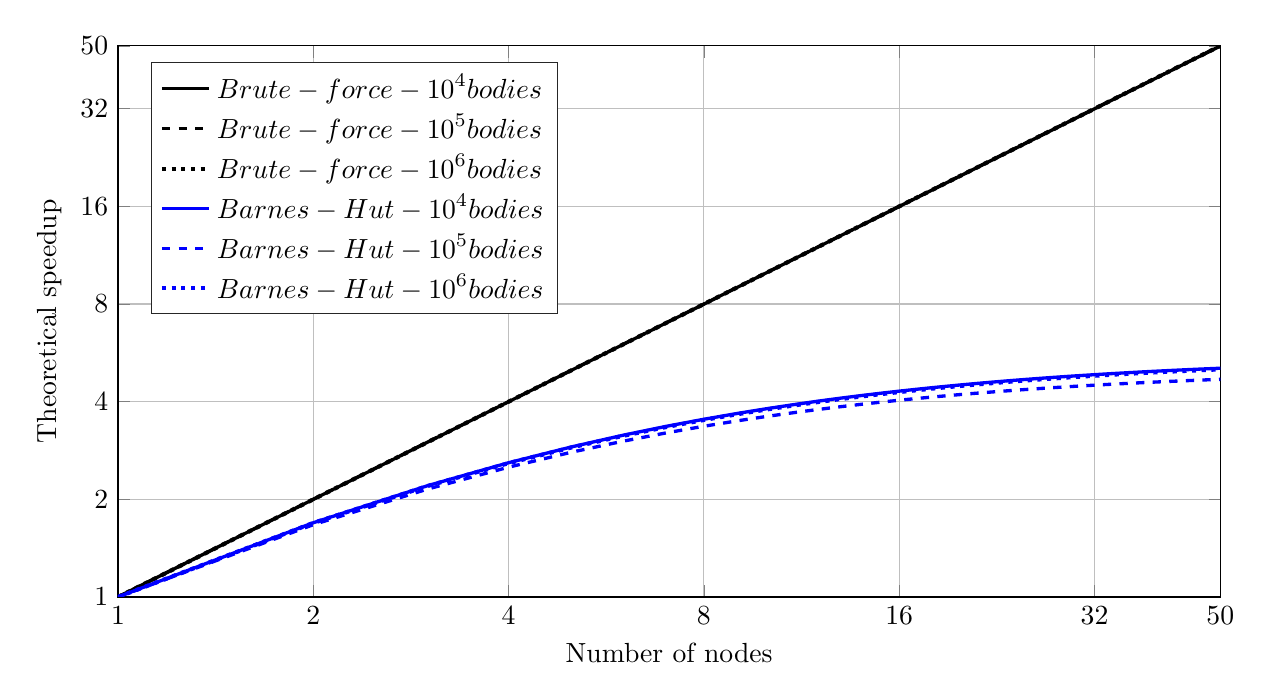
\begin{tikzpicture}

\begin{axis}[%
width=14cm,
height=7cm,
at={(0.769167in,0.484687in)},
scale only axis,
xmode=log,
xmin=1,
xmax=50,
xtick={1,2,4, 8, 16, 32, 50},
xticklabels={{1},{2},{4},{8},{16},{32}, {50}},
xminorticks=true,
xlabel={Number of nodes},
xmajorgrids,
xminorgrids,
ymode=log,
ymin=1,
ymax=50,
ytick={1,2,4, 8, 16, 32, 50},
yticklabels={{1},{2},{4},{8},{16},{32}, {50}},
yminorticks=true,
ylabel={Theoretical speedup},
ymajorgrids,
yminorgrids,
legend style={at={(0.03,0.97)},anchor=north west,legend cell align=left,align=left,draw=white!15!black}
]
\addplot [color=black,solid,line width=1.2pt]
  table[row sep=crcr]{%
1	1\\
2	1.99994667610975\\
3	2.99984003259429\\
4	3.99968007371821\\
5	4.99946680374565\\
6	5.99920022694027\\
7	6.99888034756531\\
8	7.99850716988353\\
9	8.99808069815725\\
10	9.99760093664832\\
11	10.9970678896182\\
12	11.9964815613277\\
13	12.9958419560375\\
14	13.9951490780075\\
15	14.9944029314973\\
16	15.9936035207661\\
17	16.9927508500726\\
18	17.9918449236749\\
19	18.9908857458309\\
20	19.9898733207979\\
21	20.9888076528327\\
22	21.9876887461918\\
23	22.986516605131\\
24	23.985291233906\\
25	24.9840126367717\\
26	25.9826808179827\\
27	26.9812957817933\\
28	27.979857532457\\
29	28.9783660742272\\
30	29.9768214113565\\
31	30.9752235480974\\
32	31.9735724887018\\
33	32.9718682374209\\
34	33.9701107985058\\
35	34.9683001762071\\
36	35.9664363747747\\
37	36.9645193984584\\
38	37.9625492515072\\
39	38.9605259381699\\
40	39.9584494626946\\
41	40.9563198293293\\
42	41.9541370423213\\
43	42.9519011059174\\
44	43.9496120243642\\
45	44.9472698019075\\
46	45.944874442793\\
47	46.9424259512657\\
48	47.9399243315702\\
49	48.9373695879508\\
50	49.9347617246512\\
};
\addlegendentry{$\text{Brute-force - 10}^\text{4}\text{ bodies}$};

\addplot [color=black,dashed,line width=1.2pt]
  table[row sep=crcr]{%
1	1\\
2	1.99999718001251\\
3	2.99999154004945\\
4	3.99998308012275\\
5	4.99997180024435\\
6	5.99995770042617\\
7	6.99994078068014\\
8	7.99992104101818\\
9	8.99989848145223\\
10	9.99987310199421\\
11	10.9998449026561\\
12	11.9998138834497\\
13	12.999780044387\\
14	13.99974338548\\
15	14.9997039067406\\
16	15.9996616081806\\
17	16.9996164898121\\
18	17.999568551647\\
19	18.9995177936971\\
20	19.9994642159744\\
21	20.9994078184909\\
22	21.9993486012584\\
23	22.999286564289\\
24	23.9992217075944\\
25	24.9991540311867\\
26	25.9990835350778\\
27	26.9990102192795\\
28	27.9989340838039\\
29	28.9988551286628\\
30	29.9987733538682\\
31	30.9986887594321\\
32	31.9986013453662\\
33	32.9985111116826\\
34	33.9984180583932\\
35	34.9983221855099\\
36	35.9982234930447\\
37	36.9981219810094\\
38	37.998017649416\\
39	38.9979104982764\\
40	39.9978005276025\\
41	40.9976877374064\\
42	41.9975721276998\\
43	42.9974536984947\\
44	43.9973324498031\\
45	44.9972083816368\\
46	45.9970814940079\\
47	46.9969517869282\\
48	47.9968192604096\\
49	48.9966839144641\\
50	49.9965457491035\\
};
\addlegendentry{$\text{Brute-force - 10}^\text{5}\text{ bodies}$};

\addplot [color=black,dotted,line width=1.5pt]
  table[row sep=crcr]{%
1	1\\
2	1.9999992455067\\
3	2.99999773652095\\
4	3.99999547304362\\
5	4.99999245507554\\
6	5.99998868261758\\
7	6.99998415567059\\
8	7.99997887423542\\
9	8.99997283831293\\
10	9.99996604790397\\
11	10.9999585030094\\
12	11.9999502036301\\
13	12.9999411497668\\
14	13.9999313414205\\
15	14.999920778592\\
16	15.9999094612822\\
17	16.9998973894918\\
18	17.9998845632219\\
19	18.9998709824731\\
20	19.9998566472464\\
21	20.9998415575427\\
22	21.9998257133627\\
23	22.9998091147073\\
24	23.9997917615775\\
25	24.9997736539739\\
26	25.9997547918976\\
27	26.9997351753493\\
28	27.9997148043299\\
29	28.9996936788403\\
30	29.9996717988813\\
31	30.9996491644537\\
32	31.9996257755585\\
33	32.9996016321964\\
34	33.9995767343683\\
35	34.9995510820752\\
36	35.9995246753177\\
37	36.9994975140969\\
38	37.9994695984135\\
39	38.9994409282683\\
40	39.9994115036624\\
41	40.9993813245964\\
42	41.9993503910713\\
43	42.9993187030879\\
44	43.999286260647\\
45	44.9992530637496\\
46	45.9992191123964\\
47	46.9991844065884\\
48	47.9991489463263\\
49	48.9991127316111\\
50	49.9990757624435\\
};
\addlegendentry{$\text{Brute-force - 10}^\text{6}\text{ bodies}$};

\addplot [color=blue,solid,line width=1.2pt]
  table[row sep=crcr]{%
1	1\\
2	1.6937899510075\\
3	2.20334216965291\\
4	2.59344192354659\\
5	2.90168652023547\\
6	3.15139327484974\\
7	3.3577912616699\\
8	3.53124848721009\\
9	3.67906809928399\\
10	3.80654294649019\\
11	3.91760274810478\\
12	4.01522637737897\\
13	4.10171304425647\\
14	4.17886567627005\\
15	4.24811796544492\\
16	4.31062428772729\\
17	4.36732456528899\\
18	4.41899185637153\\
19	4.46626781077842\\
20	4.50968945352666\\
21	4.54970967422904\\
22	4.58671308287264\\
23	4.62102841010838\\
24	4.6529382998322\\
25	4.68268711217689\\
26	4.71048719307112\\
27	4.73652395078827\\
28	4.76095999619283\\
29	4.7839385421459\\
30	4.80558621224844\\
31	4.8260153752877\\
32	4.84532609626958\\
33	4.86360777554752\\
34	4.88094053271128\\
35	4.89739638043212\\
36	4.91304022454\\
37	4.92793071962079\\
38	4.94212100391271\\
39	4.95565933291098\\
40	4.96858962760298\\
41	4.98095195045862\\
42	4.9927829200442\\
43	5.00411607329853\\
44	5.01498218302057\\
45	5.02540953689811\\
46	5.03542418340513\\
47	5.0450501490685\\
48	5.05430963091904\\
49	5.06322316737192\\
50	5.07180979030545\\
};
\addlegendentry{$\text{Barnes-Hut - 10}^\text{4}\text{ bodies}$};

\addplot [color=blue,dashed,line width=1.2pt]
  table[row sep=crcr]{%
1	1\\
2	1.67045595392877\\
3	2.15122262669296\\
4	2.51282529355071\\
5	2.7946831136722\\
6	3.0205556205969\\
7	3.2056163683254\\
8	3.36000997234063\\
9	3.49077610601366\\
10	3.60295297064327\\
11	3.70024139831853\\
12	3.78542098544317\\
13	3.86061994924348\\
14	3.92749537556431\\
15	3.98735675224598\\
16	4.04125256988969\\
17	4.09003226056965\\
18	4.13439129697756\\
19	4.17490456175802\\
20	4.21205139842249\\
21	4.24623466659004\\
22	4.27779541150231\\
23	4.30702428195494\\
24	4.33417050754315\\
25	4.35944902295441\\
26	4.38304617067176\\
27	4.40512430237917\\
28	4.42582551945939\\
29	4.44527473482025\\
30	4.46358219549278\\
31	4.48084557363471\\
32	4.49715170969999\\
33	4.5125780734583\\
34	4.52719399474528\\
35	4.541061705201\\
36	4.55423722401665\\
37	4.5667711142776\\
38	4.57870913143453\\
39	4.59009278143526\\
40	4.60095980286681\\
41	4.61134458491023\\
42	4.62127853086129\\
43	4.63079037531225\\
44	4.63990646174279\\
45	4.64865098616808\\
46	4.6570462115893\\
47	4.6651126572488\\
48	4.67286926607704\\
49	4.68033355320799\\
50	4.68752173801374\\
};
\addlegendentry{$\text{Barnes-Hut - 10}^\text{5}\text{ bodies}$};

\addplot [color=blue,dotted,line width=1.5pt]
  table[row sep=crcr]{%
1	1\\
2	1.691421267001\\
3	2.19800335525537\\
4	2.58512724431123\\
5	2.89059086663529\\
6	3.1377672908751\\
7	3.34188660133655\\
8	3.51329796445007\\
9	3.65927987990264\\
10	3.78510039650046\\
11	3.89466642690251\\
12	3.9909366804081\\
13	4.07619286756916\\
14	4.15222285768443\\
15	4.22044742612696\\
16	4.28200987107316\\
17	4.33784059917366\\
18	4.38870447407415\\
19	4.4352360663391\\
20	4.4779662641571\\
21	4.51734261811561\\
22	4.55374507636363\\
23	4.58749828431542\\
24	4.61888129324529\\
25	4.64813529300237\\
26	4.67546982260366\\
27	4.70106779715546\\
28	4.72508960619414\\
29	4.74767647758651\\
30	4.76895325608716\\
31	4.78903071203335\\
32	4.80800747033416\\
33	4.82597163066769\\
34	4.84300213505739\\
35	4.85916992761708\\
36	4.87453894240263\\
37	4.88916694837746\\
38	4.90310627503627\\
39	4.91640443789987\\
40	4.92910467963817\\
41	4.94124643980696\\
42	4.95286576394922\\
43	4.96399566100014\\
44	4.97466641645997\\
45	4.98490586759234\\
46	4.99473964591353\\
47	5.00419139142041\\
48	5.01328294232639\\
49	5.02203450351125\\
50	5.03046479641954\\
};
\addlegendentry{$\text{Barnes-Hut - 10}^\text{6}\text{ bodies}$};

\end{axis}
\end{tikzpicture}%
\caption{\label{fig:amdahl} Result of the  prediction from Amdahl's law of the theoretical speedup for the Brute-Force and the Barnes-Hut algorithm.}
\end{figure}

As we can see in Figure \ref{fig:amdahl}, the Brute-Force algorithms will scale almost perfectly. Therefore, we can imagine that with a very high number of processes, it will be able to surpass the Barnes-Hut algorithm. It is possible, but this will cost a lot of energy and it is expensive. So, it is better to use the Barnes-Hut algorithm. We will still have a look at the scaling of the Brute-Force algorithm to validate the theory.

\section{Strong scaling}

In this section, we want to have a look at the strong scaling of the Brute-Force and the Barnes-Hut algorithms. The strong scaling consists, in this case, of fixing the total number of bodies and running the code with a different number of processes. In order to get the speedup factor $S_p$, we divide the time $T_p$ on $p$ processes by the time $T_1$ on 1 process.
\\
We ran the code on a private server\footnote{The cluster Deneb was full. We decided to use a private bare metal server (provided by SoftLayer) for 24 hours.} Here are the specificities of the server:
\begin{itemize}
\item OS: Ubuntu 14.04, 64- bit.
\item Processor (2$\times$): 2.6GHz Intel Xeon-Haswell (E5-2690-V3-DodecaCore)
\item RAM: 8x16GB Micron 16GB DDR4 2Rx4
\item Motherboard: SuperMicro X10DRU-i+
\end{itemize}
This server allows us to run up to 48 process\footnote{Normally, we should only use 24 cores. But in order to get more results, we decided to use the hyper-threading. Therefore, the results with more than 24 cores needs to be treated carefully.} in parallel thanks to Intel's hyper-threading. We can therefore run the code with a different number of process using the same total number of bodies. Finally, we can compare it to the theoretical results, {\it i.e.} Amdahl's law. 

\subsection{Results}

\subsubsection{Brute-Force}

The results of the strong scaling for the Brute-Force algorithm are given in Figure \ref{fig:bf_strong}. We can see that the trend of the experience (blue) follows the theoretical one. For $10^4$ and $10^5$ bodies, the speedup is even better than the theoretical one. The curve for $10^6$ bodies follows closely the theoretical one. We can see a strange behaviour after 18 cores. The reason is that there is always something running in the background on a private server, therefore using 24 cores at 100\% is difficult. For a higher number of cores, the hyper-threading is not as good as real cores, therefore we can see some strange behaviour. However, we can see that the Brute-Force algorithm is highly scalable in terms of strong scaling.

\begin{figure}[H]
\centering
% This file was created by matlab2tikz.
% Minimal pgfplots version: 1.3
%
%The latest updates can be retrieved from
%  http://www.mathworks.com/matlabcentral/fileexchange/22022-matlab2tikz
%where you can also make suggestions and rate matlab2tikz.
%
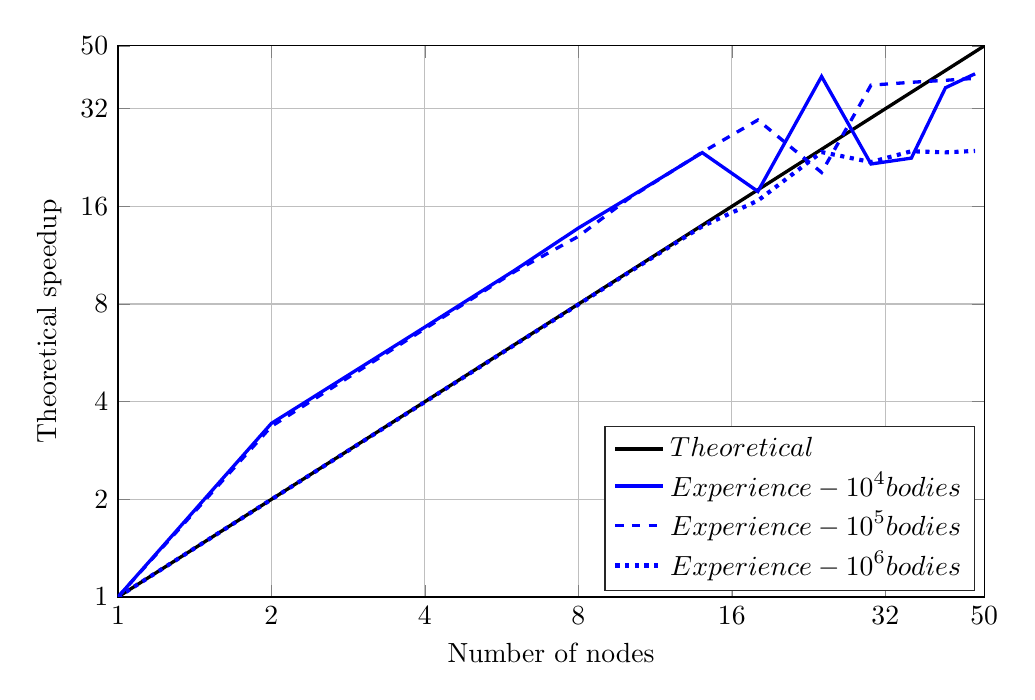
\begin{tikzpicture}

\begin{axis}[%
width=11cm,
height=7cm,
at={(0.758333in,0.48125in)},
scale only axis,
minor tick num=2,
xmode=log,
xmin=1,
xmax=50,
xtick={1,2,4, 8, 16, 32, 50},
xticklabels={{1},{2},{4},{8},{16},{32}, {50}},
xminorticks=true,
xlabel={Number of nodes},
xmajorgrids,
xminorgrids,
ymode=log,
ymin=1,
ymax=50,
ytick={1,2,4, 8, 16, 32, 50},
yticklabels={{1},{2},{4},{8},{16},{32}, {50}},
yminorticks=true,
ylabel={Theoretical speedup},
ymajorgrids,
yminorgrids,
legend style={at={(0.99,0.01)},anchor=south east,legend cell align=left,align=left,draw=white!15!black}
]
\addplot [color=black,solid,line width=1.2pt]
  table[row sep=crcr]{%
1	1\\
2	1.99994667610975\\
3	2.99984003259429\\
4	3.99968007371821\\
5	4.99946680374565\\
6	5.99920022694027\\
7	6.99888034756531\\
8	7.99850716988353\\
9	8.99808069815725\\
10	9.99760093664832\\
11	10.9970678896182\\
12	11.9964815613277\\
13	12.9958419560375\\
14	13.9951490780075\\
15	14.9944029314973\\
16	15.9936035207661\\
17	16.9927508500726\\
18	17.9918449236749\\
19	18.9908857458309\\
20	19.9898733207979\\
21	20.9888076528327\\
22	21.9876887461918\\
23	22.986516605131\\
24	23.985291233906\\
25	24.9840126367717\\
26	25.9826808179827\\
27	26.9812957817933\\
28	27.979857532457\\
29	28.9783660742272\\
30	29.9768214113565\\
31	30.9752235480974\\
32	31.9735724887018\\
33	32.9718682374209\\
34	33.9701107985058\\
35	34.9683001762071\\
36	35.9664363747747\\
37	36.9645193984584\\
38	37.9625492515072\\
39	38.9605259381699\\
40	39.9584494626946\\
41	40.9563198293293\\
42	41.9541370423213\\
43	42.9519011059174\\
44	43.9496120243642\\
45	44.9472698019075\\
46	45.944874442793\\
47	46.9424259512657\\
48	47.9399243315702\\
49	48.9373695879508\\
50	49.9347617246512\\
};
\addlegendentry{$\text{Theoretical}$};

\addplot [color=blue,solid,line width=1.2pt]
  table[row sep=crcr]{%
1	1\\
2	3.42925471046399\\
4	6.79257459044641\\
6	10.1633461651765\\
8	13.714181986027\\
10	16.9440831875905\\
14	23.4254135746757\\
18	17.7877819303264\\
24	40.2189015342734\\
30	21.6119855681537\\
36	22.5317381487344\\
42	37.132820448075\\
48	40.9948773613096\\
};
\addlegendentry{$\text{Experience - 10}^\text{4}\text{ bodies}$};

\addplot [color=blue,dashed,line width=1.2pt]
  table[row sep=crcr]{%
1	1\\
2	3.35753355073828\\
4	6.71422822208064\\
6	10.0742079403381\\
8	12.9243680954307\\
10	16.8384079627956\\
14	23.4914494193664\\
18	29.53096485438\\
24	20.3555955202194\\
30	37.823360314925\\
36	38.6004223567074\\
42	39.1471304378261\\
48	39.7049792945639\\
};
\addlegendentry{$\text{Experience - 10}^\text{5}\text{ bodies}$};

\addplot [color=blue,dotted,line width=1.5pt]
  table[row sep=crcr]{%
1	1\\
2	1.9986201271968\\
4	3.99176590621979\\
6	5.98613406977237\\
8	7.97139614687259\\
10	9.96425077095036\\
14	13.8867782682208\\
18	16.6644665756666\\
24	23.5181186183345\\
30	21.9055151110455\\
36	23.6605248632189\\
42	23.4692024900614\\
48	23.7126390881708\\
};
\addlegendentry{$\text{Experience - 10}^\text{6}\text{ bodies}$};

\end{axis}
\end{tikzpicture}%
\caption{\label{fig:bf_strong} Results of the Strong scaling for the Brute-Force algorithm. We only plot here the theoretical curve for $10^5$ bodies since the three theoretical curves are close to each other.}
\end{figure}

\subsubsection{Barnes-Hut}

The results of the strong scaling for the Barnes-Hut algorithm are given in Figure \ref{fig:bh_strong}. The experimental results follow the theoretical results. We can see that the speedup is even a bit better than the theoretical one. It comes from the fact that when computing the Amdahl's law for the Barnes-Hut algorithm, we computed some values for the average assignment and communication times. But these times can change while using a different number of processes. We can also see a strange behaviour with more than 18 cores. It is due to the same reasons as explained in the previous section. With these results, we confirm that the Barnes-Hut algorithm is not highly scalable in terms of strong scaling.

\begin{figure}[H]
\centering
% This file was created by matlab2tikz.
% Minimal pgfplots version: 1.3
%
%The latest updates can be retrieved from
%  http://www.mathworks.com/matlabcentral/fileexchange/22022-matlab2tikz
%where you can also make suggestions and rate matlab2tikz.
%
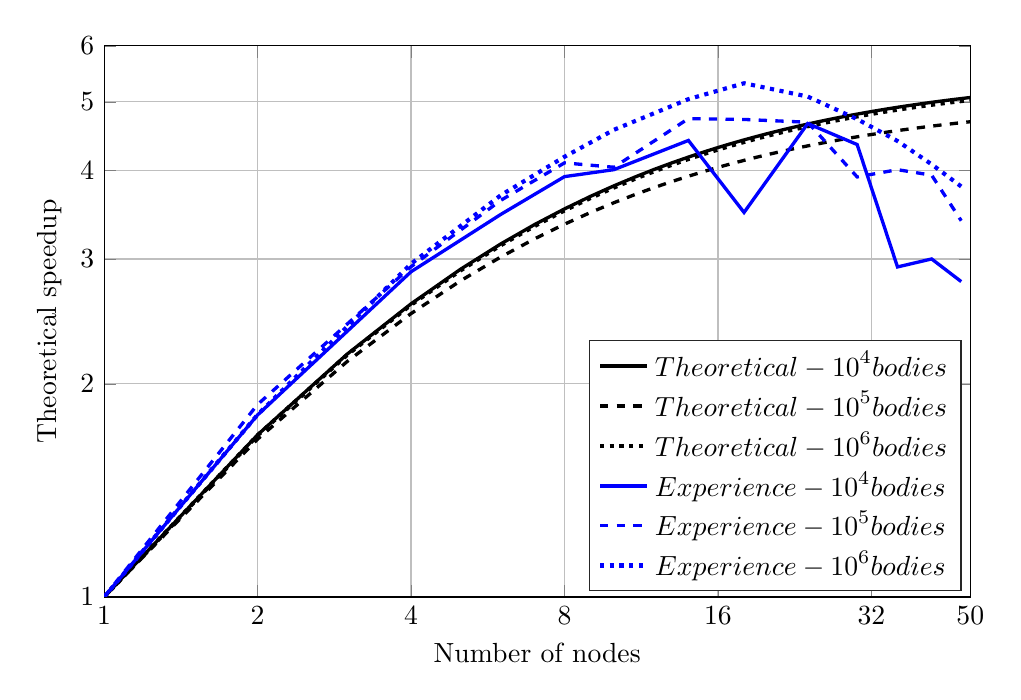
\begin{tikzpicture}

\begin{axis}[%
width=11cm,
height=7cm,
at={(0.758333in,0.48125in)},
scale only axis,
xmode=log,
xmin=1,
xmax=50,
xtick={1,2,4, 8, 16, 32, 50},
xticklabels={{1},{2},{4},{8},{16},{32}, {50}},
xminorticks=true,
xlabel={Number of nodes},
xmajorgrids,
xminorgrids,
ymode=log,
ymin=1,
ymax=6,
ytick={1,2,3,4,5,6},
yticklabels={{1},{2},{3},{4},{5},{6}},
yminorticks=true,
ylabel={Theoretical speedup},
ymajorgrids,
yminorgrids,
legend style={at={(0.99,0.01)},anchor=south east,legend cell align=left,align=left,draw=white!15!black}
]
\addplot [color=black,solid,line width=1.2pt]
  table[row sep=crcr]{%
1	1\\
2	1.6937899510075\\
3	2.20334216965291\\
4	2.59344192354659\\
5	2.90168652023547\\
6	3.15139327484974\\
7	3.3577912616699\\
8	3.53124848721009\\
9	3.67906809928399\\
10	3.80654294649019\\
11	3.91760274810478\\
12	4.01522637737897\\
13	4.10171304425647\\
14	4.17886567627005\\
15	4.24811796544492\\
16	4.31062428772729\\
17	4.36732456528899\\
18	4.41899185637153\\
19	4.46626781077842\\
20	4.50968945352666\\
21	4.54970967422904\\
22	4.58671308287264\\
23	4.62102841010838\\
24	4.6529382998322\\
25	4.68268711217689\\
26	4.71048719307112\\
27	4.73652395078827\\
28	4.76095999619283\\
29	4.7839385421459\\
30	4.80558621224844\\
31	4.8260153752877\\
32	4.84532609626958\\
33	4.86360777554752\\
34	4.88094053271128\\
35	4.89739638043212\\
36	4.91304022454\\
37	4.92793071962079\\
38	4.94212100391271\\
39	4.95565933291098\\
40	4.96858962760298\\
41	4.98095195045862\\
42	4.9927829200442\\
43	5.00411607329853\\
44	5.01498218302057\\
45	5.02540953689811\\
46	5.03542418340513\\
47	5.0450501490685\\
48	5.05430963091904\\
49	5.06322316737192\\
50	5.07180979030545\\
};
\addlegendentry{$\text{Theoretical - 10}^\text{4}\text{ bodies}$};

\addplot [color=black,dashed,line width=1.2pt]
  table[row sep=crcr]{%
1	1\\
2	1.67045595392877\\
3	2.15122262669296\\
4	2.51282529355071\\
5	2.7946831136722\\
6	3.0205556205969\\
7	3.2056163683254\\
8	3.36000997234063\\
9	3.49077610601366\\
10	3.60295297064327\\
11	3.70024139831853\\
12	3.78542098544317\\
13	3.86061994924348\\
14	3.92749537556431\\
15	3.98735675224598\\
16	4.04125256988969\\
17	4.09003226056965\\
18	4.13439129697756\\
19	4.17490456175802\\
20	4.21205139842249\\
21	4.24623466659004\\
22	4.27779541150231\\
23	4.30702428195494\\
24	4.33417050754315\\
25	4.35944902295441\\
26	4.38304617067176\\
27	4.40512430237917\\
28	4.42582551945939\\
29	4.44527473482025\\
30	4.46358219549278\\
31	4.48084557363471\\
32	4.49715170969999\\
33	4.5125780734583\\
34	4.52719399474528\\
35	4.541061705201\\
36	4.55423722401665\\
37	4.5667711142776\\
38	4.57870913143453\\
39	4.59009278143526\\
40	4.60095980286681\\
41	4.61134458491023\\
42	4.62127853086129\\
43	4.63079037531225\\
44	4.63990646174279\\
45	4.64865098616808\\
46	4.6570462115893\\
47	4.6651126572488\\
48	4.67286926607704\\
49	4.68033355320799\\
50	4.68752173801374\\
};
\addlegendentry{$\text{Theoretical - 10}^\text{5}\text{ bodies}$};

\addplot [color=black,dotted,line width=1.5pt]
  table[row sep=crcr]{%
1	1\\
2	1.691421267001\\
3	2.19800335525537\\
4	2.58512724431123\\
5	2.89059086663529\\
6	3.1377672908751\\
7	3.34188660133655\\
8	3.51329796445007\\
9	3.65927987990264\\
10	3.78510039650046\\
11	3.89466642690251\\
12	3.9909366804081\\
13	4.07619286756916\\
14	4.15222285768443\\
15	4.22044742612696\\
16	4.28200987107316\\
17	4.33784059917366\\
18	4.38870447407415\\
19	4.4352360663391\\
20	4.4779662641571\\
21	4.51734261811561\\
22	4.55374507636363\\
23	4.58749828431542\\
24	4.61888129324529\\
25	4.64813529300237\\
26	4.67546982260366\\
27	4.70106779715546\\
28	4.72508960619414\\
29	4.74767647758651\\
30	4.76895325608716\\
31	4.78903071203335\\
32	4.80800747033416\\
33	4.82597163066769\\
34	4.84300213505739\\
35	4.85916992761708\\
36	4.87453894240263\\
37	4.88916694837746\\
38	4.90310627503627\\
39	4.91640443789987\\
40	4.92910467963817\\
41	4.94124643980696\\
42	4.95286576394922\\
43	4.96399566100014\\
44	4.97466641645997\\
45	4.98490586759234\\
46	4.99473964591353\\
47	5.00419139142041\\
48	5.01328294232639\\
49	5.02203450351125\\
50	5.03046479641954\\
};
\addlegendentry{$\text{Theoretical - 10}^\text{6}\text{ bodies}$};

\addplot [color=blue,solid,line width=1.2pt]
  table[row sep=crcr]{%
1	1\\
2	1.80713496852145\\
4	2.87873543044448\\
6	3.46853470902353\\
8	3.92262444207154\\
10	4.01145474426364\\
14	4.41106854023671\\
18	3.49046119963774\\
24	4.66022547019529\\
30	4.35277619408911\\
36	2.92403879940567\\
42	3.00083166872478\\
48	2.78813677860674\\
};
\addlegendentry{$\text{Experience - 10}^\text{4}\text{ bodies}$};

\addplot [color=blue,dashed,line width=1.2pt]
  table[row sep=crcr]{%
1	1\\
2	1.8695639507855\\
4	2.92631062444475\\
6	3.63149384737242\\
8	4.10094373594427\\
10	4.04283600141889\\
14	4.73510091840613\\
18	4.72262035762503\\
24	4.67998551474486\\
30	3.91772658535315\\
36	4.01121144765421\\
42	3.9405887654349\\
48	3.39801052272871\\
};
\addlegendentry{$\text{Experience - 10}^\text{5}\text{ bodies}$};

\addplot [color=blue,dotted,line width=1.5pt]
  table[row sep=crcr]{%
1	1\\
2	1.80881495681558\\
4	2.95406384722919\\
6	3.69182300939317\\
8	4.18305650236037\\
10	4.56653622350815\\
14	5.04484661802744\\
18	5.31238799354336\\
24	5.08700788234988\\
30	4.72731230334919\\
36	4.40282539455343\\
42	4.08160969253081\\
48	3.79849135185379\\
};
\addlegendentry{$\text{Experience - 10}^\text{6}\text{ bodies}$};

\end{axis}
\end{tikzpicture}%
\caption{\label{fig:bh_strong} Results of the Strong scaling for the Barnes-Hut algorithm.}
\end{figure}

\section{Weak scaling}

In this section, we present the weak scaling. The weak scaling consists of fixing the number of bodies per process and changing the number of processes. Then, to obtain the efficiency $E_p$, we divide the time $T_1$ on 1 process by the time $T_p$ on $p$ process.
\\
We ran the code on a private laptop\footnote{The cluster Deneb was still full at that time. The time limit for private server, described in the previous section, was over.} Here are the specificities of the laptop:
\begin{itemize}
\item Laptop: Dell XPS 15 L502X
\item OS: Linux Mint 17.3 Cinnamon 64-bit.
\item Processor: Intel Core i7-2760QM CPU @ 2.40GHz x 4
\item RAM: 2x4GB Micron 4GB DDR3
\end{itemize}
This laptop is old and doesn't have a lot of cores (4 cores for 8 processes with Intel's hyper-threading). Nevertheless, we can grasp the concept of weak scaling. We must be careful while comparing the results with the previous section since we used a different machine.

\subsection{Results}

\subsubsection{Brute-Force}

For the weak scaling, we expect a graph with a very shallow slope, {\it i.e.} the efficiency stays around 1. The results for the Brute-Force algorithm is given in Figure \ref{fig:bf_weak}. In this case, we can see that the mean iteration time becomes bigger and bigger. Therefore, the efficiency drops down with a larger number of processes. This is quite surprising compared to the good strong scaling results of this algorithm. To analyse the the weak scaling, let us fix the bodies per process to $N$. If we have $p$ processes, the complexity of the main loop becomes $\mathcal{O}(\frac{pN}{p}\times pN) = \mathcal{O}(p\times N^2)$. This is because we only divide the number of bodies in the first \verb+for+ loop and not in the second. With this complexity, as the number of processes increases, so does the computation time and, therefore, the efficiency decreases.
\begin{figure}[H]
\centering
% This file was created by matlab2tikz.
% Minimal pgfplots version: 1.3
%
%The latest updates can be retrieved from
%  http://www.mathworks.com/matlabcentral/fileexchange/22022-matlab2tikz
%where you can also make suggestions and rate matlab2tikz.
%
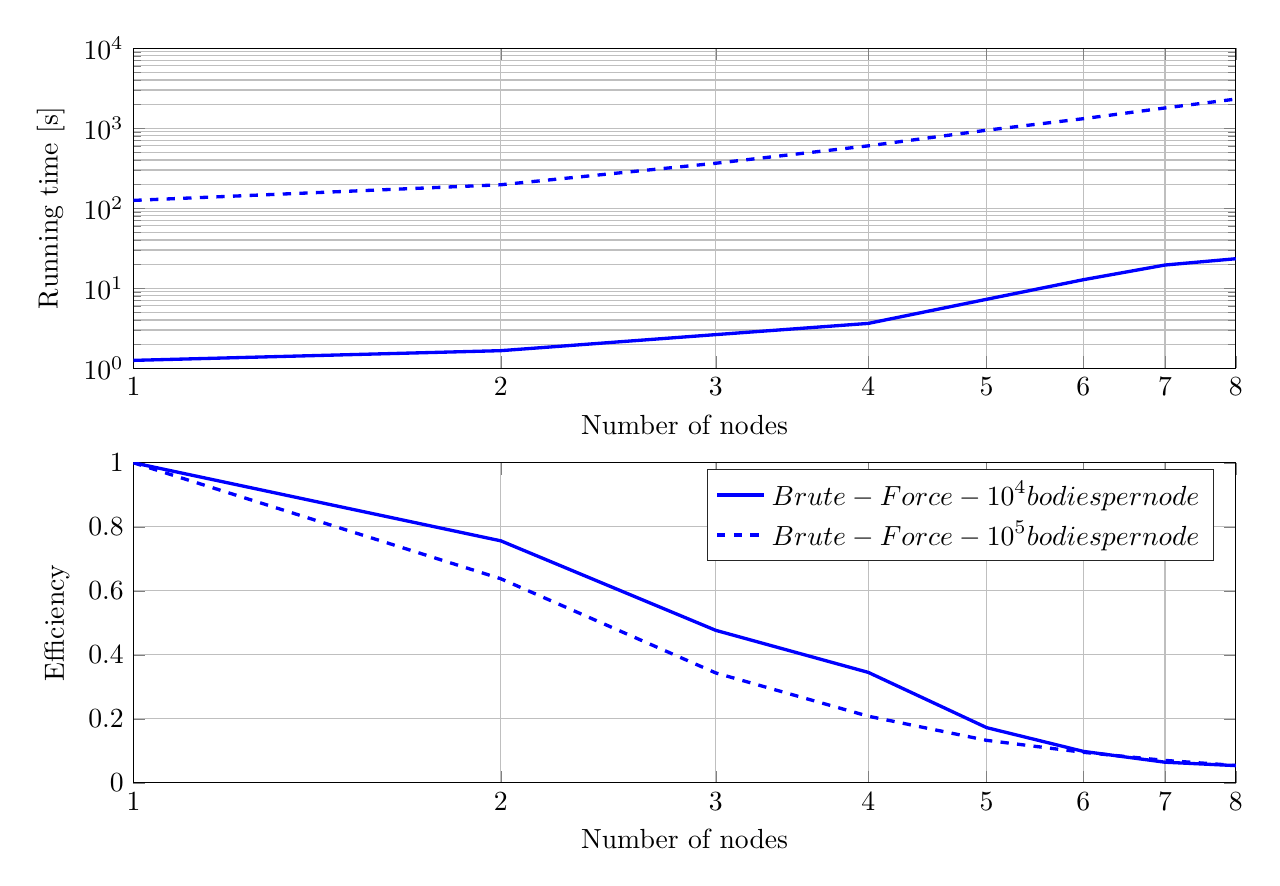
\begin{tikzpicture}

\begin{axis}[%
width=14cm,
height=1.6in,
at={(0.758333in,0.542131in)},
scale only axis,
xmode=log,
xmin=1,
xmax=8,
xminorticks=true,
xlabel={Number of nodes},
xmajorgrids,
xminorgrids,
xtick={1, 2, 3, 4, 5, 6, 7, 8},
xticklabels={{1},{2},{3},{4},{5},{6},{7},{8}},
ymin=0,
ymax=1,
ylabel={Efficiency},
ymajorgrids,
legend style={legend cell align=left,align=left,draw=white!15!black}
]
\addplot [color=blue,solid,line width=1.2pt]
  table[row sep=crcr]{%
1	1\\
2	0.756022222489609\\
3	0.476306460007734\\
4	0.344895238110588\\
5	0.17231894047816\\
6	0.0981318273010437\\
7	0.0643015717878828\\
8	0.0536375400360533\\
};
\addlegendentry{$\text{Brute-Force - 10}^\text{4}\text{ bodies per node}$};

\addplot [color=blue,dashed,line width=1.2pt]
  table[row sep=crcr]{%
1	1\\
2	0.637555427058201\\
3	0.343172333025313\\
4	0.208015206665949\\
5	0.132620712503118\\
6	0.095214562576354\\
7	0.0699260175960599\\
8	0.0541372092748112\\
};
\addlegendentry{$\text{Brute-Force - 10}^\text{5}\text{ bodies per node}$};

\end{axis}

\begin{axis}[%
width=14cm,
height=1.6in,
at={(0.758333in,2.615169in)},
scale only axis,
xmode=log,
xmin=1,
xmax=8,
xminorticks=true,
xlabel={Number of nodes},
xtick={1,2,3, 4, 5, 6, 7, 8},
xticklabels={{1},{2},{3},{4},{5},{6},{7},{8}},
xmajorgrids,
xminorgrids,
ymode=log,
ymin=1,
ymax=10000,
yminorticks=true,
ylabel={Running time [s]},
ymajorgrids,
yminorgrids
]
\addplot [color=blue,solid,line width=1.2pt,forget plot]
  table[row sep=crcr]{%
1	1.25145425759091\\
2	1.65531411691818\\
3	2.62741399218182\\
4	3.62850546863636\\
5	7.26243008527273\\
6	12.7527866545455\\
7	19.4622654282727\\
8	23.3316862919091\\
};
\addplot [color=blue,dashed,line width=1.2pt,forget plot]
  table[row sep=crcr]{%
1	125.071203889818\\
2	196.173067598091\\
3	364.455965279091\\
4	601.259907361818\\
5	943.07443784\\
6	1313.57221527455\\
7	1788.62186335727\\
8	2310.26322865909\\
};
\end{axis}
\end{tikzpicture}%
\caption{\label{fig:bf_weak} Results of the Weak scaling for the Brute-Force algorithm. The graph above is the mean iteration time in function of the number of process. The graph below is the efficiency in function of the number of process.}
\end{figure}

\subsubsection{Barnes-Hut}

The results for the Barnes-Hut algorithm are given in Figure \ref{fig:bh_weak}. We can see that we have the same behaviour as for the Brute-Force algorithm. We can think in a similar way as for the Brute-Force algorithm. The complexity of the algorithm is $\mathcal{O}(n\log n)$. Therefore, if we have $N$ bodies per process and $p$ process, we will have a complexity of $\mathcal{O}(\frac{pN}{p}\times\log(pN)) = \mathcal{O}(N\log(pN))$. We can clearly see that the running time will increase as the number of process increase. However, we should have a smaller increase than the Brute-Force algorithm. But we would need to redo the experience on more nodes to make sure we can observe this behaviour.

\begin{figure}[H]
\centering
% This file was created by matlab2tikz.
% Minimal pgfplots version: 1.3
%
%The latest updates can be retrieved from
%  http://www.mathworks.com/matlabcentral/fileexchange/22022-matlab2tikz
%where you can also make suggestions and rate matlab2tikz.
%
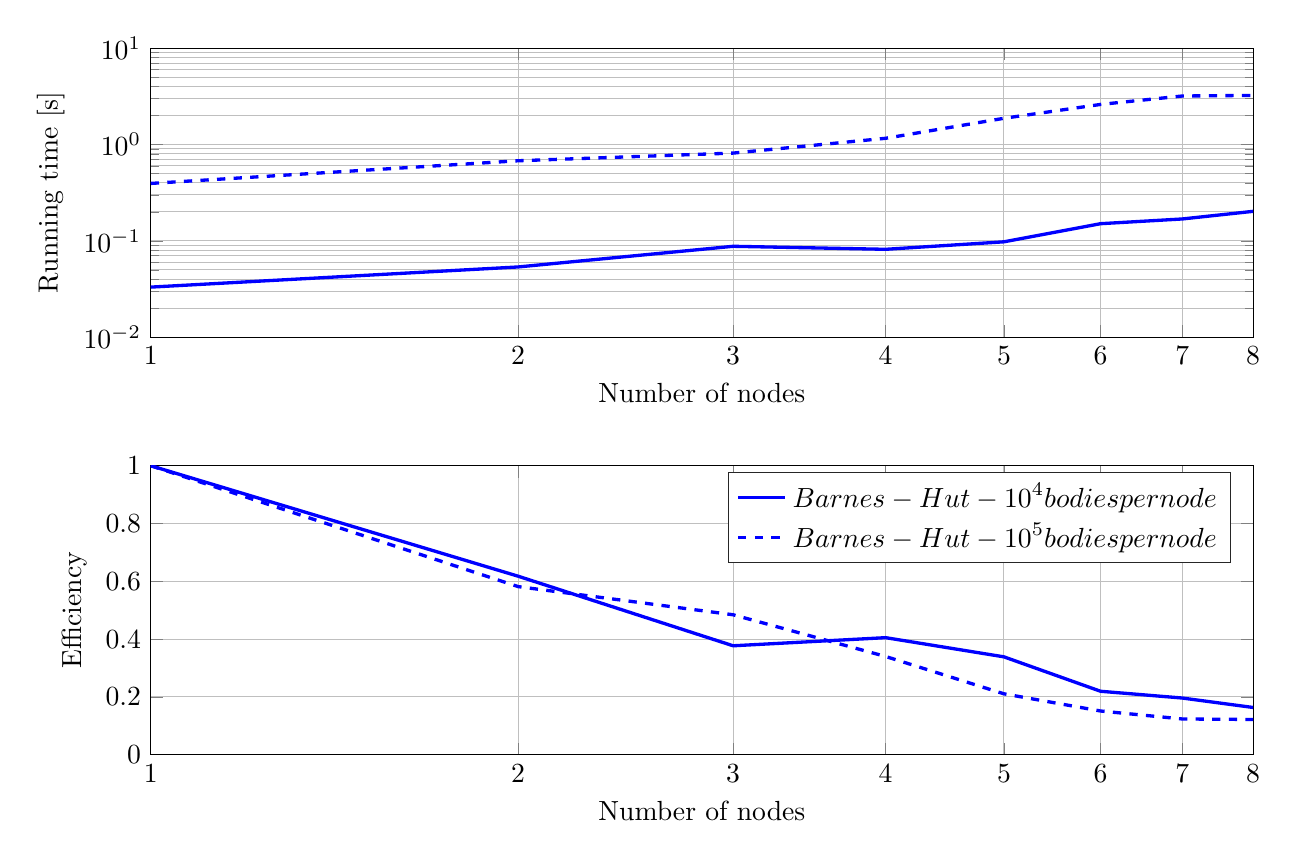
\begin{tikzpicture}

\begin{axis}[%
width=14cm,
height=1.445033in,
at={(0.769167in,2.630748in)},
scale only axis,
xmode=log,
xmin=1,
xmax=8,
xminorticks=true,
xlabel={Number of nodes},
xmajorgrids,
xminorgrids,
xtick={1,2,3, 4, 5, 6, 7, 8},
xticklabels={{1},{2},{3},{4},{5},{6},{7},{8}},
ymode=log,
ymin=0.01,
ymax=10,
yminorticks=true,
ylabel={Running time [s]},
ymajorgrids,
yminorgrids
]
\addplot [color=blue,solid,line width=1.2pt,forget plot]
  table[row sep=crcr]{%
1	0.03308295392\\
2	0.0535573495098039\\
3	0.0877561541372549\\
4	0.0816696460392157\\
5	0.0976765590196078\\
6	0.150651544509804\\
7	0.168636937058824\\
8	0.202365228823529\\
};
\addplot [color=blue,dashed,line width=1.2pt,forget plot]
  table[row sep=crcr]{%
1	0.394341795484314\\
2	0.677898941568627\\
3	0.814232577647059\\
4	1.15994181019608\\
5	1.87087138627451\\
6	2.60626458431373\\
7	3.18709408627451\\
8	3.23189081568628\\
};
\end{axis}

\begin{axis}[%
width=14cm,
height=1.445033in,
at={(0.769167in,0.542903in)},
scale only axis,
xmode=log,
xmin=1,
xmax=8,
xtick={1,2,3, 4, 5, 6, 7, 8},
xticklabels={{1},{2},{3},{4},{5},{6},{7},{8}},
xminorticks=true,
xlabel={Number of nodes},
xmajorgrids,
xminorgrids,
ymin=0,
ymax=1,
ylabel={Efficiency},
ymajorgrids,
legend style={legend cell align=left,align=left,draw=white!15!black}
]
\addplot [color=blue,solid,line width=1.2pt]
  table[row sep=crcr]{%
1	1\\
2	0.617710813227306\\
3	0.376987280780977\\
4	0.405082616669043\\
5	0.338699010817517\\
6	0.219599168582351\\
7	0.19617857449854\\
8	0.163481414827691\\
};
\addlegendentry{$\text{Barnes-Hut - 10}^\text{4}\text{ bodies per node}$};

\addplot [color=blue,dashed,line width=1.2pt]
  table[row sep=crcr]{%
1	1\\
2	0.581711773397705\\
3	0.484311001930025\\
4	0.339966877664021\\
5	0.210779745939442\\
6	0.15130535781276\\
7	0.123730829655321\\
8	0.122015816119264\\
};
\addlegendentry{$\text{Barnes-Hut - 10}^\text{5}\text{ bodies per node}$};

\end{axis}
\end{tikzpicture}%
\caption{\label{fig:bh_weak} Results of the Weak scaling for the Barnes-Hut algorithm. The graph above is the mean iteration time in function of the number of process. The graph below is the efficiency as function of the number of processes.}
\end{figure}

\section{Conclusion}

In this project, we tested two algorithms on the n-Body Gravitational problem: the basic Brute-Force algorithm and the powerful Barnes-Hut algorithm. It was very interesting to compare these two algorithms because we could see that the slowest algorithm, Brute-Force, was more scalable than the fastest algorithm. The interesting fact is that even if we use a lot of process, this algorithm will never be as fast as the Barnes-Hut algorithm. This is a really interesting fact because it teaches us that sometimes developing a good algorithm is far more interesting than using an old and slow algorithm on a powerful cluster. It is even more ecological since we will use less nodes. 


\section{Budget}

In this section, we want to present a resource budget for a huge experience. This simulation will use $10^8$ bodies. We want to run it for 2000 time steps but we will only write the positions of the bodies every 5 time steps. 

\subsection{Computing power}

As we saw, the Barnes-Hut algorithm has a complexity of $\mathcal{O}(n\log n)$. Using the times in Table \ref{tab:amdahl} (and more experience not showed in this report) and assuming that the time of the iteration follows $\beta\times n\log n$, we can estimate $\beta\simeq 0.33\cdot 10^{-6}$. Therefore, we can estimate the time required for one iteration with one process and $10^8$ bodies: $t\simeq 600~[s]$. Hence, the total time will be around 14 days: $\frac{2000\times 600}{3600\times 24} \simeq 14~$[days]. We would like to reduce this to less than a week, therefore we would require a speed up of around three\footnote{Writing the bodies in a file will take a lot of time, therefore it is better to use a higher speedup.}. Figure \ref{fig:bh_strong} shows us that we would need 6 nodes.

\subsection{Raw storage}

Writing the data of $10^6$ bodies for one time step takes $50~[MB]$ on the hard drive. It is a linear scale with respect to the number of bodies. Therefore, writing the data of $10^8$ bodies will take $5~[GB]$. Since, we want to print the data every 5 time steps for 2000 time steps, this means that we will write 400 times. Therefore, we will need $2~[TB]$ of space on the hard drive. 
\\
The RAM has also been tested. For $10^6$ bodies, it takes around $600~[MB]$. Therefore, for $10^8$ bodies, we would need around $60~[GB]$.

\subsection{Grand Total}

\begin{center}
\begin{tabular}{| l | l |}
	\hline
	Total number of requested cores & 6--10~[cores] \\
	\hline
	Minimum total memory & 64~[GB] \\
	\hline
	Maximum total memory & 128~[GB] \\
	\hline
	Temporary disk space for a single run & 2~[TB] \\
	\hline
	Permanent disk space for the entire project & 4~[TB] \\
	\hline
	Communications & Pure MPI \\
	\hline
	License & own code (BSD) \\
	\hline
	Code publicly available ? & Yes \\
	\hline
	Library requirements & None \\
	\hline
	Architectures where code ran & Intel 64 \\
	\hline
\end{tabular}
\end{center}

\begin{thebibliography}{1}

\bibitem{grav} \href{https://en.wikipedia.org/wiki/Newton's\_law\_of\_universal\_gravitation}{Wikip\'edia - Newton's law of universal gravitation}

\bibitem{bh} \href{http://http.cs.berkeley.edu/~demmel/cs267/lecture26/lecture26.html}{Berkley - CS267: Lecture 24, Apr 11 1996: Fast Hierarchical Methods for the N-body Problem, Part 1}

\bibitem{c++} Stroustrup B.,{\em Programming -- Principles and Practice Using C++}, Addison-Wesley, May 2014

\bibitem{mpi} The MPI Forum, {\em MPI: A Message-Passing Interface Standard}, Technical Report, 1994

\end{thebibliography}

\end{document}
